\documentclass[a4paper,UKenglish,cleveref,autoref,thm-restate,authorcolumns]{lipics-v2019}

\usepackage[dvipsnames]{xcolor}
\usepackage[utf8]{inputenc}
\usepackage{url}
\usepackage{todonotes}
\usepackage{amssymb}
\usepackage[fleqn]{amsmath}
\usepackage{amsbsy}
\usepackage{mathbbol}
\usepackage{mathtools}
\usepackage[many]{tcolorbox}
\bibliographystyle{plainurl}

\usepackage{hyperref}
%%
%% For section renaming in autoref
\addto\extrasUKenglish{%
\renewcommand{\sectionautorefname}{\S}%
\renewcommand{\subsectionautorefname}{\S}%
\def\exampleautorefname{Ex.}% 
\renewcommand{\figureautorefname}{Fig.}%
}

% Two column itemize
\usepackage{multicol}

% Example code
\usepackage{listings}

% Diagrams
\usepackage{tikz}

% Mathbb doesn't support digits
\usepackage{bbm}

% Less margins around figures
\usepackage{changepage}

% Inference rules
\usepackage{mathpartir}

% TODO notes -- TODO: remove
\usepackage{todonotes}

% Do not use italics in definitions and theorems
\theoremstyle{definition}
\newtheorem{nidefinition}{Definition}
\newtheorem{nitheorem}{Theorem}
\newtheorem{nilemma}{Lemma}

% No line numbers
\nolinenumbers

% Abbreviations
\newcommand{\lambdacalc}{$\lambda$-calculus}
\newcommand{\picalc}{$\pi$-calculus}
\newcommand{\Picalc}{$\pi$-Calculus}

% Typing rules
\newcommand{\stacked}[1]{\mprset{flushleft} \inferrule*{}{#1}}
\newcommand{\datatype}[2]{{\mprset{fraction={===}} \inferrule{#1}{#2}}}

\newcommand{\type}[1]{\textcolor{BlueViolet}{\operatorname{#1}}}
\newcommand{\constr}[1]{\textcolor{BurntOrange}{\operatorname{#1}}}
\newcommand{\func}[1]{\textcolor{OliveGreen}{\operatorname{#1}}}

% Constructors
\newcommand{\PO}{\constr{\mathbb{0}}}
\newcommand{\comp}[2]{#1 \; \constr{\parallel} \; #2}
\newcommand{\new}{\constr{\boldsymbol{\nu}} \;}
\newcommand{\send}[2]{#1 \; \constr{\langle} \; #2 \;\constr{\rangle} \;}
\newcommand{\sendp}[2]{#1 \; \constr{\langle} \; #2 \; \constr{\rangle} \; . \;}
\newcommand{\recv}[1]{#1 \; \constr{\mathbb{()}} \;}
\newcommand{\recvp}[2]{#1 \; \constr{(} \; #2 \; \constr{)} \; . \; }
\newcommand{\suc}{\constr{\scriptstyle 1+}}
\newcommand{\unit}{\constr{\mathbbm{1}}}
\newcommand{\base}[1]{\constr{B[} \; #1 \; \constr{]}}
\newcommand{\channel}[2]{\constr{C[} \; #1 \; \constr{;} \; #2 \; \constr{]}}
\newcommand{\comma}{\; \constr{,} \;}

% Functions
\newcommand{\subst}[3]{#1 \; \func{[} \; #3 \; \func{\mapsto} \;#2 \; \func{]}}
\newcommand{\op}[3]{#1 \; \func{\coloneqq} \; #2 \; \func{\cdot} \; #3}
\newcommand{\opsquared}[3]{#1 \, \func{\coloneqq} \, #2 \, \func{\cdot^2} \, #3}
\newcommand{\opctx}[3]{#1 \, \func{\coloneqq} \, #2 \, \func{\otimes} \, #3}
\newcommand{\zero}{\func{0\cdot}}
\newcommand{\one}{\func{1\cdot}}
\newcommand{\li}{\func{\ell_i}}
\newcommand{\lo}{\func{\ell_o}}
\newcommand{\lz}{\func{\ell_{\o}}}
\newcommand{\lio}{\func{\ell_{\#}}}

% Types
\newcommand{\Set}{\type{SET}}
\newcommand{\reduce}[1]{\; \type{\longrightarrow}_{#1} \;}
\newcommand{\types}[4]{#1 \; \type{;} \; #2 \; \type{\vdash} \; #3 \; \type{\triangleright} \; #4}
\newcommand{\contains}[6]{#1 \; \type{;} \; #2 \; \type{\ni}_{#3} \; #4 \; \type{;} \; #5 \; \type{\triangleright} \; #6}
\newcommand{\containsusage}[4]{#1 \; \type{\ni}_{#2} \; #3 \; \type{\triangleright} \; #4}
\newcommand{\Var}{\type{VAR}}
\newcommand{\Process}{\type{PROCESS}}
\newcommand{\Unused}{\type{UNUSED}}
\newcommand{\PreCtx}{\type{PRECTX}}
\newcommand{\Ctx}{\type{CTX}}
\newcommand{\Type}{\type{TYPE}\;}
\newcommand{\Idx}{\type{IDX}\;}
\newcommand{\Idxs}{\type{IDXS}}
\newcommand{\Usage}{\type{USAGE}}
\newcommand{\N}{\type{\mathbb{N}}}
\newcommand{\Channel}{\type{CHANNEL}}
\newcommand{\Rec}{\type{REC}}
\newcommand{\Algebra}{\type{ALGEBRA}}
\newcommand{\eq}[1]{\; \type{=}_{#1} \;}
\newcommand{\eqeq}{\; \type{\equiv} \;}
%%%%%%%%%%%%%%%%%%%%%%%%%%%%%%%%%%%%%%%%%%%%%%%%%%%%%%%%%%%%%%%%%%%
\title{$\pi$ with leftovers: \\ a mechanisation in Agda}
\titlerunning{$\pi$ with leftovers: all mechanisation in Agda}
\author{Uma Zalakain}{University of Glasgow, Scotland}
       {u.zalakain.1@research.gla.ac.uk}{https://orcid.org/0000-0002-3268-9338}{}
\author{Ornela Dardha}{University of Glasgow, Scotland}
       {ornela.dardha@glasgow.ac.uk}{https://orcid.org/0000-0001-9927-7875}{}
\authorrunning{U. Zalakain and O. Dardha}
\Copyright{Uma Zalakain and Ornela Dardha}
\begin{CCSXML}
<ccs2012>
<concept>
<concept_id>10003752.10003753.10003761.10003764</concept_id>
<concept_desc>Theory of computation~Process calculi</concept_desc>
<concept_significance>300</concept_significance>
</concept>
</ccs2012>
\end{CCSXML}
\ccsdesc[300]{Theory of computation~Process calculi}
\keywords{pi-calculus, linear types, leftover typing, concurrency, mechanisation, Agda}
\supplement{\url{https://github/umazalakain/typing-linear-pi}}
\acknowledgements{We want to thank Erika Kreuter, Wen Kokke, James Wood, Guillaume Allais, Bob Atkey, and Conor McBride for their thoughts, patience, work, education and camaraderie.}
\funding{Supported by the UK EPSRC grant EP/K034413/1, ``From Data Types to Session Types: A Basis for Concurrency and Distribution'' (ABCD), and by the EU HORIZON 2020 MSCA RISE project 778233
  ``Behavioural Application Program Interfaces'' (BehAPI).}
%%%%%%%%%%%%%%%%%%%%%%%%%%%%%%%%%%%%%%%%%%%%%%%%%%%%%%%%%%%%%%%%%%%

\begin{document}

\maketitle

\begin{abstract}
  The \picalc{} is a computational model for communication and concurrency.
  The \emph{linear} \picalc{} is a typed version of the \picalc{} where channels must be used exactly once.
  It is an underlying theoretical and practical framework on top of which more advanced types and theories are built, including \emph{session types} \cite{H93,THK94,HVK98}.
  Linearity is key for type safety in session communication.

  We present the \emph{first} full mechanisation in Agda of a \picalc{} with \emph{linear}, \emph{gradual} and \emph{shared} types, all under the same unified framework.
  While linearity is key for type safety in communication-centric programming, gradual and shared types are needed to model real-world software systems.
  
  We present the syntax, semantics, type system and corresponding type safety properties.
  For the first time in the \picalc{}, we use leftover typing \cite{Allais2018a} to encode our typing rules in a way that propagates linearity constraints into process continuations.
  We generalise the algebras on multiplicities, allowing the developer to choose a mix of linear, gradual and shared typing.
  We provide framing, weakening and strengthening proofs that we then use to prove subject congruence.
  We show that the type system is stable under substitution and prove subject reduction.
%
  Our formalisation is fully mechanised in Agda \cite{Zalakain2020Agda}.
\end{abstract}

\todo{spellcheck}
\todo{make sure all citations are there}

%%%%%%%%%%%%%%%%%%%%%%%%%%%%%%%%%%%%%%%%%%%%%%%%%%%%%%%%%%%%%%%%%%%
\section{Introduction}
\todo{highlight that we can talk about a resource even if it has been exhausted (e.g. we can send 0 multiplicities of a channel over another channel}
We live in a concurrent world where any given state is often interactively computed by a myriad of parties --- people, machines, processors, services, networks.
As humans, we aim to model, predict, and build such interactive systems; as mathematicians, abstraction is our tool of choice to do so.
\todo{rename gradual to something else...}
\todo{replace judgment with judgement everywhere!}
\todo{Theorem to Thm. Definiton to Def. when referencing.}

The \picalc{} \cite{MilnerPW92,Milner99} is the most successful computational model for communication and concurrency.
It abstracts over the details of concurrent processing and boils the interactions down to the sending and receiving of data over communication channels.
Notably, it features channel mobility: channels themselves are first order values, and can therefore be transmitted.
The \picalc{} has been a foundation for the design and implementation of programming languages for concurrency, such as Pict \cite{Pierce} and (more recently) Go \cite{Golang}.
At the state-of-the-art, the \picalc{} features a wide plethora of types \cite{K07}: basic types, linear types, types for liveness properties (such as deadlock freedom, livelock freedom or termination), and most notably, session types. This makes the \picalc{} a fully-fledged tool for modelling and verification of concurrent and distributed systems.

In a parallel track, J.-Y. Girard's development of linear logic \cite{Girard87} in the early '90s opened new avenues in computing science by introducing \emph{linear types} for (functional) programming languages \cite{Curry-Howard,Wadler90,Bernardy2018}.
Linear type systems guarantee that resources are used \emph{exactly once}.
Enforcing ``no duplicating'' and ``no discarding'' of resources via linearity allows for resource-aware programming and more efficient implementations \cite{Wadler90}.
Later on, linearity inspired unique types (as in Clean \cite{BarendsenS96}) and ownership types (as in Rust \cite{MatsakisK14}).

The \picalc{} also benefited from the linearity wave of the early '90s.
Kobayashi et al. \cite{KPT96} defined the {linear} \picalc{}, a typed version of the \picalc{} where the linear type system restricts the usage of channels to exactly once.
%
In the meantime, with the rise of \emph{session types} \cite{H93,THK94,HVK98} linearity acquired a different flavour in the \picalc{}.
Session types are a type formalism used in communication-centric programming.
In session types, linearity ensures that a channel is owned by exactly one communicating participant, whilst the channel itself is used multiple times as per its session type.
Linearity in session types is the key ingredient that guarantees type safety.

Recent work has pushed the linear \picalc{} into the spotlight again \cite{KPT96}, thanks to an encoding of session types into linear types \cite{DardhaGS12,Dardha14,DardhaGS17}.
This encoding not only has theoretical benefits in terms of the expressivity of session types and the reusability of theoretical results from the linear \picalc{}, but it is useful at a practical level too.
The encoding has been used as a technique to implement session types in mainstream programming languages such as OCaml \cite{Padovani17} and Scala \cite{ScalasY16,ScalasDHY17}.
This allows us to use the linear \picalc{} as an underlying theoretical and practical framework on top of which session types can be built.

Considering the relevance of the \picalc{} and of linearity in modelling concurrent and distributed systems, in this paper we focus our research on both and go beyond.

\emph{We present the first full mechanisation in Agda of a \picalc{} with linear, gradual and shared types, all under the same unified framework.}

We do so by defining a specification for an algebra on \emph{multiplicities} (how many times a channel can be used) and use it to apply leftover typing (following Allais \cite{Allais2018a}) to the \picalc{}.
The developer is able to choose any mix of algebras for the type system --- as long as they comply with the specification.
Ultimately, we can exploit this formalisation as a unified framework for type safe distributed modelling and programming with a variety of type systems, and build on top of it more advanced types, theories and languages.
In particular, while linearity is needed for type safety in communication-centric programming, gradual and shared types are needed to model real-world systems.

\subsection{Contributions}
\begin{enumerate}
\item \textbf{Formalisation of the syntax and the semantics of the \picalc{}}:
 \begin{itemize}
   \item \textbf{Syntax}: \autoref{syntax} uses type level de Bruijn indices \cite{deBruijn1972} to introduce a syntax that is \emph{well-scoped by construction}: every free variable is accounted for in the type of the process that uses it.
   
   \item \textbf{Semantics}: \autoref{semantics} provides an operational semantics for the \picalc{}, prior to any typing.
   This operational semantics is given as a reduction relation on processes (\autoref{operational-semantics}).
   The reduction relation tracks at the type level the channel the communication occurs on, so that this information can then be used to state subject reduction --- aka type preservation (\autoref{subject-reduction}).
   The reduction relation is defined modulo structural congruence (\autoref{structural-congruence}) --- a relation that acts as a quotient type that removes unnecessary syntactic minutiae introduced by the syntax of the \picalc{}.
 \end{itemize}
  
  \item \textbf{Leftover typing for the \picalc{} with linear, gradual and shared types}:
  \autoref{type-system} provides the type system for a resource-aware \picalc{}.
  \begin{itemize}
    \item \textbf{Algebras on multiplicities}: The user can provide \emph{resource-aware} algebras, which are then applied to the type system (\autoref{multiplicities}).
    Linear types, gradual types and shared types are all instances of the same resource-aware algebra, giving rise to three different type systems under the same framework.
    Any \emph{partial commutative monoid} that is \emph{functional}, \emph{cancellative} and has a minimal element is a valid such algebra.
    
    Multiple algebras can be simultaneously used in a single type system --- usage contexts keep information about what algebra to use on which element (\autoref{contexts}).
    This allows for type systems combining linear, gradual and shared types.
    
    \item \textbf{\picalc{} with leftovers}: Our type system uses \emph{leftover typing} to model the resource-aware \picalc{} (\autoref{leftover-typing}).
    This approach adds a leftover usage context to the typing judgments.
    Typing derivations take the resources of their input usage context, consume some of them, and leave the rest as leftovers in the output usage context.
    One of the benefits of this technique is that it removes the need for extrinsic context splits, which are rendered unnecessary.
  \end{itemize}
  \item \textbf{Machine verified proofs of subject reduction and auxiliary theorems}:
  \autoref{type-safety} details the type safety properties of our \picalc{} with leftovers.
  Leftover typing allows \emph{framing} (\autoref{thm:framing}), \emph{weakening} (\autoref{thm:weakening}) and \emph{strengthening} (\autoref{thm:strengthening}) theorems to be stated.
  We use these to prove \emph{subject congruence} (\autoref{subject-congruence}), and together with \emph{substitution} (\autoref{substitution}), to prove \emph{subject reduction} (\autoref{subject-reduction}).  

  \item \textbf{Fully mechanised formalisation available in Agda}:
  This work has been fully mechanised in Agda and is publicly available in our GitHub repository \cite{Zalakain2020Agda}.

\end{enumerate}


\subsection{Notation}
%%%%%%%%%%%%%%%%%%%%%%%%%%%%%%%%%%%%%%%%%%%%%%%%%%%%%%%%%%%%%%%%%%%
\autoref{fig:notation} illustrates the notation used in this paper.
\begin{figure}[h]
  \begin{mathpar}
    \datatype
    { }
    {\type{\N} : \Set}
    \; \textsc{Nat}

    \inferrule
    { }
    {\constr{0} : \type{\N}}

    \inferrule
    {n : \type{\N}}
    {\suc n : \type{\N}}
  \end{mathpar}
  \caption{Notation used in this paper.}
  \label{fig:notation}
\end{figure}

Data type definitions ($\type{\N}$) use double lines and index-free synonyms (\textsc{Nat}) as rule names (for ease of reference).
We otherwise use constructor names ($\constr{0}$ and $\suc$) to name our typing rules.
Universe levels and universe polymorphism are omitted for brevity --- all our types are of type $\Set$.
Implicit arguments are mentioned by type definitions but omitted in constructors.

We use colours to further distinguish the different entities in this paper.
$\type{TYPES}$ are blue violet (uppercased, with indices as subscripts), $\constr{constructors}$ are burnt orange, $\func{functions}$ are olive green, variables are black, and some constructor names are overloaded --- and disambiguated by context.

%%%%%%%%%%%%%%%%%%%%%%%%%%%%%%%%%%%%%%%%%%%%%%%%%%%%%%%%%%%%%%%%%%%
\section{Syntax}
\label{syntax}
\begin{figure}[h]
  \begin{subfigure}{1\textwidth}
    \begin{mathpar}
      \datatype
      {n : \N}
      {\Var_n : \Set}
      \; \textsc{Var}

      \inferrule
      {n : \N}
      {\constr{0} : \Var_{\suc n}}

      \inferrule
      {x : \Var_n}
      {\suc x : \Var_{\suc n}}

      \datatype
      {n : \N}
      {\Process_n : \Set}
      \; \textsc{Process}
    \end{mathpar}
  \end{subfigure}
  \begin{subfigure}[t]{.3\textwidth}
    \begin{equation*}
      \begin{split}
        P,Q ::=      & \; \PO                \\ 
                    |& \; (\new{}x) \; P       \\ 
                    |& \; \comp{P}{Q}        \\ 
                    |& \; \recvp{x}{y} P \\ 
                    |& \; \sendp{x}{y} P 
      \end{split}
    \end{equation*}
    \caption{Ill-scoped grammar with names.}
    \label{fig:syntax-names}
  \end{subfigure}
  \hspace{.05\textwidth}
  \begin{subfigure}[t]{.65\textwidth}
    \begin{equation*}
      \begin{split}
        \Process_n ::=& \; \PO_n               &&\text{(inaction)}   \\ 
        |& \; \new{} \Process_{\suc n}         &&\text{(restriction)}          \\ 
        |& \; \comp{\Process_n}{\Process_n}    &&\text{(parallel)} \\ 
        |& \; \recv{\Var_n}{}\Process_{\suc n} &&\text{(input)}                \\ 
        |& \; \send{\Var_n}{\Var_n}\Process_n  &&\text{(output)}                  
      \end{split}
    \end{equation*}
    \caption{Well-scoped grammar with type-level de Bruijn indices.}
    \label{fig:syntax}
  \end{subfigure}
  \caption{}
\end{figure}

Let $x, y,\ldots$ range over \emph{variables} (including channel names) and $P, Q,\ldots$ over processes.
The syntax of the \picalc{} \cite{Sangio01} is given by the grammar in \autoref{fig:syntax-names}.
Process $\PO$ denotes the terminated process, where no operations can further occur.
Process $(\new{}x)\; P$ creates a new channel $x$ bound with scope $P$.
Process $\comp{P}{Q}$ is the parallel composition of processes $P$ and $Q$.
Processes $\recvp{x}{y} P$ and $\sendp{x}{y} P$ denote respectively the input and output processes of a variable $y$ over a channel $x$, with continuation $P$.

Scope restriction $(\new{}x) \; P$ and input $\recvp{x}{y} \; P$ are \emph{binders}, they are the only constructs which introduce bound names --- $x$ and $y$ in $P$, respectively.
In order to mechanise the \picalc{} syntax in Agda, we need to deal with bound names in continuation processes.
Names are cumbersome to mechanise: inserting a new variable into a context means proving that its name differs from all other variable names in context.
Instead, we use de Bruijn indices \cite{deBruijn1972}, where a natural number $n$ (aka \emph{index}) is used to refer to the variable introduced $n$ binders ago --- hence binders no longer introduce names.
\begin{example}
  \begin{equation*}
    \begin{split}
      & (\new{}x ) && (\comp {\recvp{x}{y} && \sendp{y}{a} && \PO} {(\new{} y) && (\sendp{x}{y} && \recvp{y}{z} && \PO)})
      && \text{names}
      \\
      & \new{} && (\comp {\recv{0} && \send{0}{a} && \PO} {\new{} && (\send{1}{0} && \recv{0} && \PO)})
      && \text{de Bruijn indices}
      \\
    \end{split}
  \end{equation*}
\end{example}
That is, terms at different \emph{depths} use different indices to refer to the same binding.

A variable occurring under $n$ binders can refer to other $n$ possible variables.
References outside of that range are meaningless.
It is useful to rule out these ill-scoped nonsensical terms syntactically.
In \autoref{fig:syntax}, we do so by introducing the indexed family of types $\Var_n$: for all naturals $n$, the type $\Var_n$ has $n$ distinct elements.
We index processes according to their \emph{depth}: for all naturals $n$, a process of type $\Process_n$ contains variables that can refer to $n$ distinct elements.
Every time we go under a binder, we increase the index of the continuation process, allowing the variable references within it to refer to one more thing.

%%%%%%%%%%%%%%%%%%%%%%%%%%%%%%%%%%%%%%%%%%%%%%%%%%%%%%%%%%%%%%%%%%%
\section{Semantics}
\label{semantics}
Thanks to our well-scoped grammar in \autoref{fig:syntax}, the semantics of our language can now be defined on the totality of the syntax.
We start by defining structural congruence in \autoref{structural-congruence} and then the reduction relation in \autoref{operational-semantics}.

%%%%%%%%%%%%%%%%%%%%%%%%%%%%%%%%%%%%%%%%%%%%%%%%%%%%%%%%%%%%%%%%%%%
\subsection{Structural Congruence}
\label{structural-congruence}

We define the base cases of a structural congruence relation \textsc{StructCong} $\eqeq$ in \autoref{fig:struct-cong-base}.
Its congruent equivalence closure \textsc{Equals} $\eq{}$ is defined in \autoref{app:struct}.

\begin{figure}[h]
\begin{mathpar}
  \datatype
  { }
  {P \eqeq Q : \Set}
  \; \textsc{StructCong}

  \inferrule
  { }
  {\constr{comp-assoc} : \comp{P}{(\comp{Q}{R})} \eqeq \comp{(\comp{P}{Q})}{R}}

  \inferrule
  { }
  {\constr{comp-sym} : \comp{P}{Q} \eqeq \comp{Q}{P}}
  
  \inferrule
  { }
  {\constr{comp-end} : \comp{P}{\PO_n} \eqeq P}
  
  \inferrule
  { }
  {\constr{scope-end} : \new \PO_{\suc n} \eqeq \PO_n}
  
  \inferrule
  {uQ : \Unused_0 \; Q}
  {\constr{scope-ext} : \new (\comp{P}{Q}) \eqeq \comp{(\new P)}{\func{lower}_{\constr{0}} \; \; Q \; uQ}}

  \inferrule
  { }
  {\constr{scope-comm} : \new \new P \eqeq \new \new \func{swap}_{\constr{0}} \; P}
\end{mathpar}
\caption{Base cases of structural congruence.}
\label{fig:struct-cong-base}
\end{figure}

The first three rules ($\constr{comp}-$*) state associativity, symmetry, and $\PO$ as the neutral element of parallel composition, respectively.
The last three ($\constr{scope}-$*) state garbage collection, scope extrusion and commutativity of restrictions, respectively.

In $\constr{scope-ext}$ the type $\Unused_i \; Q$ is an inductive proof asserting that the variable index $i$ does not appear neither in the inputs nor in the outputs of $Q$.
The function $\func{lower}_i \; Q \; uQ$ traverses $Q$ decrementing every index bigger than $i$.
In $\constr{scope-comm}$ the function $\func{swap}_i \; P$ traverses $P$ (of type $\Process_{\suc \suc n}$) and swaps variable references $i$ and $\suc i$.
In all the above, $i$ is incremented every time we go under a binder.
  
%%%%%%%%%%%%%%%%%%%%%%%%%%%%%%%%%%%%%%%%%%%%%%%%%%%%%%%%%%%%%%%%%%%
\subsection{Reduction Relation}
\label{operational-semantics}

The operational semantics of the \picalc{} is defined by a reduction relation \textsc{Reduces} $\reduce{c}$ indexed by the channel $c$ on which communication occurs (\autoref{fig:reduction}).
We keep track of channel $c$ so we can state subject reduction (\autoref{subject-reduction}).
We distinguish between channels created inside a process ($\constr{internal}$) and channels created outside ($\constr{external}\ i$, where $i$ is the de Bruijn index of the variable).

In rule $\constr{comm}$, parallel processes reduce when they communicate over a common channel with index ${i}$.
As a result of that communication, the continuation of the input process $P$ has all the references to its most immediate variable substituted with references to $\suc j$, the variable sent by the output process $\send{i}{j}{Q}$.
After substitution, $\subst{P}{\suc j}{\constr{0}}$ is \emph{lowered} --- all variable references are decreased by one (to do so, we apply \autoref{lm:subst-unused} in \autoref{app:lemmas} to obtain a proof $\Unused_{\constr{0}} \; (\subst{P}{\suc j}{\constr{0}})$).
Reduction is closed under parallel composition (rule $\constr{par}$), restriction (rule $\constr{res}$) and structural congruence (rule $\constr{struct}$) 
--- notably, not under input nor output, as doing so would not preserve the sequencing of actions \cite{Sangio01}.


In $\constr{res}$, we use a $\func{dec}$ function to decrement the index of channel $c$ as we wrap processes $P$ and $Q$ inside a binder.
This $\func{dec}$ function saturates at $\constr{internal}$: wrapping an internally reducing process with a binder will result in an internally reducing process.


\begin{figure}[h]
\begin{mathpar}
  \datatype
  {n : \N}
  {\Channel_n : \Set}
  \; \textsc{Channel}

  \inferrule
  { }
  {\constr{internal} : \Channel_n}

  \inferrule
  {i : \Var_n}
  {\constr{external} \; i : \Channel_n}

  \datatype
  {c : \Channel_n \\ P \; Q : \Process_n}
  {P \reduce{c} Q : \Set}
  \; \textsc{Reduces}

  \inferrule
  {i \; j : \Var_n \\ P : \Process_{\suc n} \\ Q : \Process_n}
  {\constr{comm} : \comp{\recv{i}P}{\send{i}{j}{Q}} \reduce{\constr{external} \; i} \comp{\func{lower}_{\constr{0}} \; (\subst{P}{\suc j}{\constr{0}}) \; uP'}{Q}}

  \inferrule
  {red : P \reduce{c} P'}
  {\constr{par} \; red : \comp{P}{Q} \reduce{c} \comp{P'}{Q}}

  \inferrule
  {red : P \reduce{c} Q}
  {\constr{res} \; red : \new P \reduce{\func{dec}\; c} \new Q}

  \inferrule
  {eq : P \eq{r} P' \\ red : P' \reduce{c} Q}
  {\constr{struct} \; eq \; red : P \reduce{c} Q}
\end{mathpar}
\caption{Operational semantics indexed by the channel over which reduction occurs.}
\label{fig:reduction}
\end{figure}

%%%%%%%%%%%%%%%%%%%%%%%%%%%%%%%%%%%%%%%%%%%%%%%%%%%%%%%%%%%%%%%%%%%
\section{Resource-aware Type System}
\label{type-system}

In \autoref{multiplicities} we characterise a usage algebra for our type system.
It defines how resources are \emph{split} in parallel composition and \emph{consumed} in input and output.
We define typing and usage contexts in \autoref{contexts}.
We provide a type system for a resource-aware \picalc{} in \autoref{leftover-typing}.

\subsection{Multiplicities and Capabilities}
%%%%%%%%%%%%%%%%%%%%%%%%%%%%%%%%%%%%%%%%%%%%%%%%%%%%%%%%%%%%%%%%%%%
\label{multiplicities}

In the linear \picalc{} each channel has an input and an output \emph{capability}, and each capability has a given \emph{multiplicity} of 0 (exhausted) or 1 (available).
We generalise over this notion by defining an algebra that is satisfied by linear, gradual and shared types alike.

\begin{nidefinition}[Usage algebra]
  A \emph{usage algebra} is a ternary relation $\op{x}{y}{z}$, that is \emph{partial}, \emph{functional}, \emph{cancellative}, \emph{associative}, and \emph{commutative}.
  It has a \emph{neutral element} $\zero$ that is absorbed on either side, and that is also \emph{minimal}.
  It has an element $\one$ that is used to count inputs and outputs.
  \autoref{fig:multiplicities} uses a terniary relation to model such an algebra as a record $\Algebra_C$ on a carrier $C$.

  \begin{figure}[h]
  \begin{equation*}
  \begin{aligned}
    &\zero                  &:{} &                 &        & C \\
    &\one                   &:{} &                 &        & C \\
    &\op{\_}{\_}{\_}        &:{} &                 &        & C \to C \to C \to \Set \\
    &\func{\cdot-compute}  &:{} &\forall y z       & \to \; & \type{DEC} \; (\type{\exists} x  \; (\op{x}{y}{z})) \\
    &\func{\cdot-unique}   &:{} &\forall x x' y z  & \to \; & \op{x'}{y}{z} \to \op{x}{y}{z} \to x' \equiv x \\
    &\func{\cdot-unique^l} &:{} &\forall x y y' z  & \to \; & \op{x}{y'}{z} \to \op{x}{y}{z} \to y' \equiv y \\
    &\func{0\cdot-min^l}   &:{} &\forall y z       & \to \; & \op{\zero}{y}{z} \to y \equiv \zero \\
    &\func{\cdot-id^l}     &:{} &\forall x         & \to \; & \op{x}{\zero}{x} \\
    &\func{\cdot-comm}     &:{} &\forall x y z     & \to \; & \op{x}{y}{z} \to \op{x}{z}{y} \\
    &\func{\cdot-assoc}    &:{} &\forall x y z u v & \to \; & \op{x}{y}{z} \to \op{y}{u}{v} \to \type{\exists} w  \; (\op{x}{u}{w} \times \op{w}{v}{z})
  \end{aligned}
  \end{equation*}
  \caption{
    Usage algebra $\Algebra_C$ on a carrier $C$.
    We use $\forall$ for universal quantification.
    The dependent product $\type{\exists}$ uses the value of its first argument in the type of its second.
    The type $\type{DEC} \; P$ is a witness of either $P$ or $P \to \type{\bot}$, where $\type{\bot}$ is the empty type with no constructors.
  }
  \label{fig:multiplicities}
  \end{figure}
\end{nidefinition}

\begin{note}
  \label{note:linearity}
  We will often work with pairs of input and output multiplicities.
  We use the notation $\type{C}^{\func{2}}$ to stand for a $\type{C} \constr{\times} \type{C}$ tuple of input and output multiplicities, respectively.
  We use $\opsquared{x}{y}{z}$ to stand for a monoidal operation on pairs of multiplicities -- where the algebraic laws are lifted element-wise.

  Henceforth, we use $\lz$ to denote the pair $(0 \comma 0)$ for a channel which cannot be used any further, $\li$ for the pair $(1 \comma 0)$ for a channel to be used in input exactly once, $\lo$ for $(0 \comma 1)$ for a channel to be used in output exactly once, and $\lio$ for $(1 \comma 1)$, for a channel to be used exactly once in input and exactly once in output.
  This notation was originally used in the linear \picalc{} \cite{KPT96,Sangio01}.
\end{note}

Linear, gradual and shared types are all defined as an instance of our usage algebra.
Their use in typing derivations is illustrated in \autoref{example-derivations}.
\begin{description}
  \item [Linear]
    The carrier is a type with two trivial elements $\constr{zero}$ and $\constr{one}$.
    The monoidal operation has the element $\constr{zero}$ as neutral on both sides, and the element $\constr{one}$ splitting into $\constr{one}$ and $\constr{zero}$ (or $\constr{zero}$ and $\constr{one}$), and is uninhabited otherwise.
    All the properties of the algebra follow trivially.
    As an example, the multiplicity pair $\ell_i$ is represented as $(\constr{one} \comma \constr{zero})$.

    \item [Gradual]
    The carrier is the type of natural numbers.
    The element $\zero$ corresponds to 0, and $\one$ to 1.
    The partial monoid $\op{x}{y}{z}$ is defined exactly when $x = y + z$.
    All other properties of the algebra follow from the algebraic rules for the addition of natural numbers.
    As an example, we use $(5 \comma 3)$ to represent the multiplicities of a channel that is able to input 5 times and output 3 times.

    \item [Shared]
    The carrier is a type with a single trivial constructor $\constr{\omega}$.
    Both $\zero$ and $\one$ are instantiated to $\constr{\omega}$.
    The relation $\op{\constr{\omega}}{\constr{\omega}}{\constr{\omega}}$ is inhabited.
    All the properties of the algebra follow trivially.
    Shared channels have multiplicities $(\constr{\omega} \comma \constr{\omega})$, which they will forever preserve.
\end{description}

%%%%%%%%%%%%%%%%%%%%%%%%%%%%%%%%%%%%%%%%%%%%%%%%%%%%%%%%%%%%%%%%%%% 
\subsection{Typing Contexts}
\label{contexts}

We use indexed sets of usage algebras to allow several usage algebras to coexist in our type system with leftovers (\autoref{leftover-typing}).
\begin{nidefinition}[Indexed set of usage algebras]
  An \emph{indexed set of usage algebras} is a nonempty type $\Idx$ of indices together with an interpretation $\Usage$ of indices into types, and an interpretation $\type{ALGEBRAS}$ of indices into usage algebras (\autoref{fig:indexed-multiplicities}).
  \begin{figure}[h]
    \begin{equation}
      \begin{split}
        &\Idx               &:{} &\Set \\
        &\type{\exists IDX} &:{} &\Idx \\
        &\Usage             &:{} &\Idx \to \Set \\
        &\type{ALGEBRAS}    &:{} &(idx : \Idx) \to \Algebra_{\Usage_{idx}}
      \end{split}
    \end{equation}
    \caption{Indexed set of usage algebras.}
    \label{fig:indexed-multiplicities}
  \end{figure}
\end{nidefinition}

We keep typing contexts ($\PreCtx$, in \autoref{fig:prectx}) and usage contexts ($\Ctx$ in \autoref{fig:ctx}) separate.
The former are preserved throughout a typing derivation; the latter are transformed as a result of input, output, and context splits.

\begin{nidefinition}[Types and length-indexed typing contexts]
  A \emph{Type} is either a unit type ($\unit$), a base type ($\base{n}$) or a channel type ($\channel{t}{x}$) defined in \autoref{fig:prectx}.
  
  A \emph{length-indexed typing context} $\PreCtx_n$, is defined by the last row of rules in \autoref{fig:prectx}.
  A typing context is either empty $[]$ or the result of appending a type $t$ to an existing context$\gamma$.
  \begin{figure}[h]
  \begin{mathpar}
    \datatype
    { }
    {\Type : \Set}
    \; \textsc{Type}
  
    \inferrule
    { }
    {\unit : \Type}

    \inferrule
    {n : \N}
    {\base{n} : \Type}
  
    \inferrule
    {t : \Type \\ \stacked{idx : \Idx \\\\ x : \Usage_{idx}^{\func{2}}}}
    {\channel{t}{x} : \Type}
  \end{mathpar}
  
  \begin{mathpar}
    \datatype
    {n : \N}
    {\PreCtx_n : \Set}
    \; \textsc{PreCtx}
  
    \inferrule
        { }
        {[] : \PreCtx_{\constr{0}}}
  
        \inferrule
            {\gamma : \PreCtx_n \\ t : \Type}
            {\gamma \comma t : \PreCtx_{\suc n}}
  \end{mathpar}
  \caption{Types and length-indexed typing contexts.}
  \label{fig:prectx}
  \end{figure}
\end{nidefinition}

The unit type $\unit$ serves as a proof of inhabitance for types.
The base type $\base{n}$ uses natural numbers as placeholders for types (the host language can then interpret the former into the latter --- e.g. $0$ as booleans, $1$ as natural numbers) so that we avoid having to deal with universe polymorphism.
The type $\channel{t}{x}$ of a channel determines what type of data ${t}$ and what usage annotations ${x}$ are sent over that channel.

Notice that our notation of channel types is similar to Kobayashi's $[t]\mathbf{chan}_{(i^{y},o^{z})}$, where $y,z$ are the multiplicities of input and output, respectively \cite{K07}.

\begin{nidefinition}[Usage contexts]
  A \emph{usage context} is a context $\Ctx_{idxs}$ of usage annotations that is indexed by a length-indexed context of indices $\Idxs_n$ (\autoref{fig:ctx}).

  A usage context is either empty $[]$ or the result or appending a usage annotation $x$ to the existing context $\Gamma$.

  \begin{figure}[h]
  \begin{mathpar}
    \datatype
    {n : \N}
    {\Idxs_n : \Set}
    \; \textsc{Idxs}
  
    \inferrule
        { }
        {[] : \Idxs_{\constr{0}}}
  
    \inferrule
        {idxs : \Idxs_n \\ idx : \Idx}
        {idxs \comma idx : \Idxs_{\suc n}}
  
    \datatype
    {idxs : \Idxs_n}
    {\Ctx_{idxs} : \Set}
    \; \textsc{Ctx}
  
    
    \inferrule
        { }
        {[] : \Ctx_{[]}}
        
    \inferrule
        {\Gamma : \Ctx_{idxs} \\ x : \Usage_{idx} ^{\func{2}}}
        {\Gamma \comma x : \Ctx_{idxs \comma idx}}
  \end{mathpar}
  \caption{Length-indexed context of carrier indices with a context of multiplicities on top.}
  \label{fig:ctx}
  \end{figure}
\end{nidefinition}


\begin{note}
  We lift the monoidal operation on usage annotations $\opsquared{x}{y}{z}$ to a monoidal operation $\opctx{\Gamma}{\Delta}{\Xi}$ on usage contexts that have a common underlying context of indices.
  All the properties of the partial monoid are trivially lifted.
\end{note}

%%%%%%%%%%%%%%%%%%%%%%%%%%%%%%%%%%%%%%%%%%%%%%%%%%%%%%%%%%%%%%%%%%% 
\subsection{Typing with Leftovers}
\label{leftover-typing}

We use \emph{leftover typing} \cite{Allais2018a} for our type system, an approach that, in addition to the usual typing context $\PreCtx_n$ and (input) usage context $\Ctx_{idxs}$, adds an extra \emph{output usage context} to the typing rules.

This output context contains the \emph{leftovers} (the unused multiplicities) of the process being typed.
These leftovers can then be used as an input to another typing derivation.
Leftover typing presents three main advantages:
\begin{itemize}
  \item \textbf{Encapsulation}:
    The transformations to the usage context (consequence of receiving and sending over a channel) are encapsulated into a variable reference judgement with both an input and an output usage context.
  \item \textbf{No context split}:
    No need for an extensional context splitting proof for parallel composition.
    Such a proof would need to construct a witness $\opctx{\Gamma_m}{\Gamma_l}{\Gamma_r}$, where $\Gamma_l \vdash P$, $\Gamma_r \vdash Q$ and $\Gamma_m \vdash \comp{P}{Q}$.
    This could be obtained through automated search --- but it is better yet not to need it.
    Leftover typing uses the leftovers of $P$ to type $Q$.
  \item \textbf{New theorems}:
    For the first time, theorems like \textbf{framing} (\autoref{thm:framing}), \textbf{weakening} (\autoref{thm:weakening}) and \textbf{strengthening} (\autoref{thm:strengthening}) can now be stated within the linear \picalc{} --- as well as gradual and shared, thanks to the presence of a leftover context.
\end{itemize}

Our type system with leftovers is composed of two typing relations: one for variable references (\autoref{def:varref}) and one for processes (\autoref{def:types}).
Both relations are indexed by a typing context $\gamma$, an input usage context $\Gamma$, and an output usage context $\Delta$ (the leftovers).

The typing judgement for variables $\contains{\gamma}{\Gamma}{i}{t}{y}{\Delta}$ asserts that ``index $i$ is of type $t$ in typing context $\gamma$, and subtracting $y$ at position $i$ from input usage context $\Gamma$ results in leftover $\Delta$''.
The typing judgement for processes $\types{\gamma}{\Gamma}{P}{\Delta}$ asserts that ``process $P$ is well-typed under typing context $\gamma$, usage input context $\Gamma$ and leftovers $\Delta$''.



\begin{nidefinition}[\textsc{VarRef}: typing variable references]
  \label{def:varref}

  The \textsc{VarRef} typing relation for variable references is presented in \autoref{fig:variable-references}.
  \begin{figure}[h]
  \begin{mathpar}
    \mprset{sep=0.5em}
  
    \datatype{
      \gamma : \PreCtx_n \\
      \stacked{
        idxs : \Idxs_n \\\\
        \Gamma : \Ctx_{idxs}} \\
      i : \Var_n \\
      t : \Type \\
      \stacked{
        idx : \Idx \\\\
        y : \Usage_{idx}^{\func{2}}} \\
      \Delta : \Ctx_{idxs}}
    {\contains{\gamma}{\Gamma}{i}{t}{y}{\Delta} : \Set}
    \; \textsc{VarRef}
  
    \inferrule
    {\opsquared{x}{y}{z}}
    {\constr{0} : \contains{\gamma \comma t}{\Gamma \comma x}{\constr{0}}{t}{y}{\Gamma \comma z}}
    
    \inferrule
    {loc_i : \contains{\gamma}{\Gamma}{i}{t}{x}{\Delta}}
    {\suc \; loc_i : \contains{\gamma \comma t'}{\Gamma \comma x'}{\suc i}{t}{x}{\Delta \comma x'}}
  \end{mathpar}
  \caption{Typing rules for variable references.}
  \label{fig:variable-references}
  \end{figure}

  The base case $\constr{0}$ splits the usage annotation $x$ of type $\Usage_{idx}$ into $y$ and $z$ (the leftovers).
  This splitting $\opsquared{x}{y}{z}$ is as per the usage algebra provided by the developer for the index $idx$.
  We use the \emph{functionality} of the monoidal relation to alleviate the user from the proof burden $\opsquared{x}{y}{z}$.
  The inductive case $\suc$ appends the type $t'$ to the typing context, and the usage annotation $x'$ to both the input and output usage contexts. 
\end{nidefinition}

\begin{example}[Channels]
  Let us illustrate the use of channels with an example.
  \begin{lstlisting}[label=lst:channels,mathescape,caption=The underscore \_ introduces an anonymous declaration immediately followed by its definition.]
  _ : $\contains{\constr{[]} \comma \channel{\unit}{\li} \comma \unit} {\constr{[]} \comma \lio \comma \lio} {\suc \; \constr{0}} {\channel{\unit}{\li}} {\li} {\constr{[]} \comma \lo \comma \lio}$
  _ = $\suc \; \constr{0}$
  \end{lstlisting}
  In \autoref{lst:channels}, the constructor $\suc$ steps under the outermost variable in the context, preserving its usage annotation $\lio$ from input to output.
  The constructor $\constr{0}$ asserts that the next variable is of type $\channel{\unit}{\li}$, and that we can split its input annotation $\lio$, taking away $\li$ and leaving leftovers $\lo$.
\end{example}

\begin{nidefinition}[\textsc{Types}: typing processes]
  \label{def:types}

  The \textsc{Types} typing relation for \picalc{} processes is presented in \autoref{fig:types}.
  
  \begin{figure}[h]
  \begin{mathpar}
    \datatype{
      \gamma : \PreCtx_n \\
      \stacked{
        idxs : \Idxs_n \\\\
        \Gamma : \Ctx_{idxs}} \\
      P : \Process_n \\
      \Delta : \Ctx_{idxs}}
    {\types{\gamma}{\Gamma}{P}{\Delta} : \Set}
    \; \textsc{Types}
    
    \inferrule
    { }
    {\constr{end} : \types{\gamma}{\Gamma}{\PO}{\Gamma}}
  
    \inferrule
    {t : \Type \\ x : \Usage_{idx}^{\func{2}} \\ y : \Usage_{idx'} \\\\
     cont : \types{\gamma \comma \channel{t}{x}}{\Gamma \comma (y \comma y) }{P}{\Delta \comma \lz}}
    {\constr{chan} \; t \; x \; y \; cont : \types{\gamma}{\Gamma}{\new P}{\Delta}}
  
    \inferrule
        {\stacked{
            chan_i : \contains{\gamma \hspace{1.2em}}{\Gamma \hspace{1.3em}}{i}{\channel{t}{x}}{\li}{\Xi} \\\\
            cont \hspace{0.6em} : \types{\gamma \comma t}{\Xi \comma x}{P \hspace{4.6em}}{\Theta \comma \lz}}}
        {\constr{recv} \; chan_i \; cont : \types{\gamma}{\Gamma}{\recv{i}{P}}{\Theta}}
  
    \inferrule
        {\stacked{
            chan_i : \contains{\gamma}{\Gamma \hspace{0.2em}}{i}{\channel{t}{x}}{\lo}{\Delta} \\\\
            loc_j \hspace{0.8em} : \contains{\gamma}{\Delta}{j}{t \hspace{3.2em}}{x \hspace{0.3em}}{\Xi} \\\\
            cont \hspace{0.6em} : \types{\gamma}{\Xi \hspace{0.3em}}{P\hspace{4.8em}}{\Theta}}}
        {\constr{send} \; chan_i \; loc_j \; cont : \types{\gamma}{\Gamma}{\send{i}{j}P}{\Theta}}
  
    \inferrule
    {l \hspace{0.3em} : \types{\gamma}{\Gamma \hspace{0.2em}}{P}{\Delta} \\\\
     r : \types{\gamma}{\Delta}{Q}{\Xi}}
    {\constr{comp} \; l \; r : \types{\gamma}{\Gamma}{\comp{P}{Q}}{\Xi}}
  \end{mathpar}
  \caption{Leftover typing for a resource-aware type system.}
  \label{fig:types}
  \end{figure}

  The inaction process in rule $\constr{end}$ does not change usage annotations.
  The scope restriction in rule $\constr{chan}$ expects three arguments: the type $t$ of data being transmitted; the usage annotation $x$ that is being transmitted; and the multiplicity $y$ given to the channel itself.
  This multiplicity $y$ is used for both input and output, so that these are balanced.
  The continuation process $P$ is provided with the new channel with usage annotation $(y \comma y)$, which it must completely exhaust.

  The input process in rule $\constr{recv}$ requires a channel $chan_i$ at index $i$ with usage $\li$ available, such that data with type $t$ and usage $x$ can be sent over it.
  Note that the index $i$ is used in the syntax of the typed process.
  We use the leftovers $\Xi$ to type the continuation process, which is also provided with the received element --- of type $t$ and multiplicity $x$ at index $\constr{0}$.
  The received element $x$ must be completely exhausted by the continuation process.

  Similarly to input, the output processes in rule $\constr{send}$ requires a channel $chan_i$ at index $i$ with usage $\lo$ available, such that data with type $t$ and usage $x$ can be sent over it.
  We use the leftover context $\Delta$ to type the continuation process, which needs an element $loc_j$ at index $j$ with type $t$ and usage $x$, as per the type of channel $chan_i$.
  The leftovers $\Xi$ are used to type the continuation process.
  Note that both indices $i$ and $j$ are used in the syntax of the typed process.
  
  Parallel composition in rule $\constr{comp}$ uses the leftovers of the left-hand process to type the right-hand process.
  By keeping track in the typing derivation of $P$ the resources it uses, we save the user from having to provide an extrinsic proof of context split.
\end{nidefinition}

\begin{example}[Typing derivation]
  \label{example-derivations}
  We will now illustrate a typing derivation of the process $\func{p}$ using linear and shared types, given in line ?? of Listing \autoref{}.

  Let $\func{\omega}$ be a shortcut for $(\one \comma \one)$ in an algebra of shared types.
  Let $\epsilon$ be the empty usage context --- where all usage annotations are $(\zero \comma \zero)$.
  To type $\func{p}$, we need a channel over which we can transmit another channel.
  We therefore create a new channel with usage annotations $(\one \comma \one)$ capable of transmitting data of type $\channel{\unit}{\func{\omega}}$, and declare (with $\li$) that we will only transmit its input capability.
  The left-hand process (line ??) is typed following its syntax.
  On the right-hand (line ??), we need the channel that is going to be sent.
  The type $\unit$ of this channel is entirely determined by the type of the channel over which it is going to be transmitted.
  Its usage annotation is $(\one \comma \one)$: we will transmit $\li$ and save $\lo$ for the continuation process.
  
  \begin{lstlisting}[mathescape]
  $\func{p}$ : $\Process_1$
  $\func{p}$ = $\new{}$
       $(\comp{\recv{\constr{0}} (\recv{\constr{0}} \PO)}$
       ${\new{} (\send{\suc \; \constr{0}} {\constr{0}} (\send{\constr{0}}{\suc \; \suc \; \constr{0}}) \; \PO)})$

  $\func{\_}$ : $\types{\constr{[]} \comma \unit}{\constr{[]} \comma \func{\omega}}{\func{p}}{\epsilon}$
  $\func{\_}$ = $\constr{chan} \; \channel{\unit}{\func{\omega}} \; \li \; \one \; (\constr{comp}$
       $(\constr{recv} \; \constr{0} \; (\constr{recv} \; \constr{0} \; \constr{end}))$
       $(\constr{chan} \; \unit \; \func{\omega} \; \one \; (\constr{send} \; (\suc \; \constr{0}) \; \constr{0} \; (\constr{send} \; \constr{0} \; (\suc \; \suc \; \constr{0}) \; \constr{end})))
       )$
  \end{lstlisting}
\end{example}


%%%%%%%%%%%%%%%%%%%%%%%%%%%%%%%%%%%%%%%%%%%%%%%%%%%%%%%%%%%%%%%%%%%
\section{Type Safety}
\label{type-safety}

\todo{intro}

\subsection{Auxiliaty Results}
\label{auxiliary-results}
%%%%%%%%%%%%%%%%%%%%%%%%%%%%%%%%%%%%%%%%%%%%%%%%%%%%%%%%%%%%%%%%%%%

\begin{nitheorem}[Framing]
  \label{thm:framing}
  The well-typedness of a process is independent of its leftover resources.
  Let $P$ be a well-typed process $\types{\gamma}{\Gamma_l}{P}{\Xi_l}$.
  Let there be a $\Delta$ such that $\opctx{\Gamma_l}{\Delta}{\Xi_l}$.
  Take arbitrary contexts $\Gamma_r$ and $\Xi_r$ such that $\opctx{\Gamma_r}{\Delta}{\Xi_r}$.
  Then $\types{\gamma}{\Gamma_r}{P}{\Xi_r}$.
\end{nitheorem}

\begin{nitheorem}[Weakening]
  \label{thm:weakening}
  Inserting a new variable into the context preserves the well-typedness of a process as long as the usage annotation of the inserted variable is preserved as a leftover.

  Let $\func{insert}_i$ insert an element into a context at position $i$ --- for simplicity, we use it both to insert types into typing contexts and usage annotations into usage contexts.
  Let $P$ be a well-typed process such that $\types{\gamma}{\Gamma}{P}{\Xi}$.
  Then lifting every variable greater than or equal to $i$ in $P$ is well-typed under $\types{\func{insert}_i \; t \; \gamma}{\func{insert}_i \; x \; \Gamma}{\func{lift}_i \; P}{\func{insert}_i \; x \; \Xi}$.
\end{nitheorem}

\begin{nitheorem}[Strengthening]
  \label{thm:strengthening}
  Removing an unused variable preserves the well-typedness of a process.

  Let $\func{delete}_i$ delete the element at position $i$ from a context --- for simplicity, we use it both to delete types from typing contexts and usage annotations from usage contexts.
  Let $P$ be a well-typed process such that $\types{\gamma}{\Gamma}{P}{\Xi}$.
  Let $i$ be a variable index not mentioned by $P$, such that $\Unused_i \; P$.
  Then lowering every variable greater than or equal to $i$ in $P$ is well-typed under $\types{\func{delete}_i \; \gamma}{\func{delete}_i \; \Gamma}{\func{lower}_i \; P}{\func{delete}_i \; \Xi}$.
\end{nitheorem}

\begin{remark}
  It is possible for the usage annotations of a variable $i$ within a process $P$ to be preserved as leftovers, yet for the variable $i$ to be mentioned within $P$ --- $P$ can choose to send $\lz$ usage annotations of $i$ over a channel.
\end{remark}

\begin{nitheorem}[Swapping]
  \label{thm:swapping}
  Swapping two variables preserves the well-typedness of a process.
  Let $\func{swap}_i$ be a function that swaps variables $i$ and $\suc i$.
  For simplicity, we overload $\func{swap}$ and use it to swap types in a typing context, multiplicities in a usage context, and variable references in a process.
  \todo{}
  Let $P$ be a well-typed process such that $\types{\gamma}{\Gamma}{P}{\Xi}$.
  Then $\types{\func{swap}_i \; \gamma}{\func{swap}_i \; \Gamma}{\func{swap}_i \; P}{\func{swap}_i \; \Xi}$.
\end{nitheorem}

\begin{remark}
  We limit ourselves to the swapping of adjacent variables $i$ and $\suc i$.
  Doing so is enough to prove subject reduction.
  More generally, any two variables can be swapped by performing a series of adjacent variable swappings.
\end{remark}

\begin{proof}
  All the above theorems are by induction on \textsc{Process} and \textsc{Var}.
  For details, refer to the mechanisation in Agda \cite{Zalakain2020Agda}.
\end{proof}


\subsection{Subject Congruence}
%%%%%%%%%%%%%%%%%%%%%%%%%%%%%%%%%%%%%%%%%%%%%%%%%%%%%%%%%%%%%%%%%%%
\label{subject-congruence}

\begin{nitheorem}[Subject congruence]
  \label{thm:subject-congruence}
  Applying structural congruence rules to a well-typed process preserves its well-typedness.
  That is, if $P \eq{r} Q$ and $\types{\gamma}{\Gamma}{P}{\Xi}$, then $\types{\gamma}{\Gamma}{Q}{\Xi}$.
\end{nitheorem}

\todo{considering that Equals is in the appendix, you cannot do induction on something that is not defined in the main text. Bring the proof in the appendix. Maybe briefly comment on the proof here}
\begin{proof}
  By induction on \textsc{Equals}.
  The base cases under $\constr{struct}$ (and their symmetric variants under $\constr{sym}$) are the nontrivial ones.
  For those, we proceed by induction on \textsc{StructCong}:
  \begin{itemize}
    \item
      The case $\constr{comp-assoc}$ is trivial: leftover typing is naturally associative.
    \item
      In the $\constr{comp-sym}$ case for a process $\comp{P}{Q}$, we need framing (\autoref{thm:framing}) to shift the output context of $P$ to the one of $Q$; and the input context of of $Q$ to the one of $P$.
      The point at which $Q$ and $P$ join in $\comp{Q}{P}$ will no longer be the same.
    \item
      The case $\constr{comp-end}$ is trivial: the typing rule for a process $\PO$ has the same input and output contexts.
    \item
      In the $\constr{scope-end}$ case, we show that the usage annotation of the newly created channel must be $\lz$, making the proof trivial.
      In the opposite direction, we instantiate the newly created channel to a type $\unit$ and a usage annotation $\lz$..
    \item
      In the $\constr{scope-ext}$ case for a process $\new \comp{P}{Q}$, we use \autoref{lm:types-unused} to show that $P$ preserves the usage annotations of the unused variable.
      We then use strengthening (\autoref{thm:strengthening}) to delete the unused variable from $P$, and compose the result with typing derivation on $Q$ wrapped in $\constr{chan}$.
      In the reverse direction, we weaken (\autoref{thm:weakening}) $P$ so that it accepts the additional variable.
      We then use \autoref{lm:lower-lift} to show that lowering and then lifting $P$ results in $P$.
    \item
      In the $\constr{scope-comm}$ case, we use swapping (\autoref{thm:swapping}).
      In the reverse direction, we use swapping and then \autoref{lm:swap-swap} to show that swapping two elements in $P$ twice leaves $P$ unchanged.
  \end{itemize}
\end{proof}

\subsection{Substitution}
\label{substitution}
%%%%%%%%%%%%%%%%%%%%%%%%%%%%%%%%%%%%%%%%%%%%%%%%%%%%%%%%%%%%%%%%%%%

\autoref{thm:subst-generalization} proves a generalized version of substitution, where the substitution $\subst{P}{j}{i}$ is on any variable $i$.
\autoref{thm:substitution} instantiates the generalized version to the concrete case where $i$ is $\constr{0}$, as required by subject reduction.

\begin{figure}[h]
  \begin{subfigure}{.5\textwidth}
    \centering
    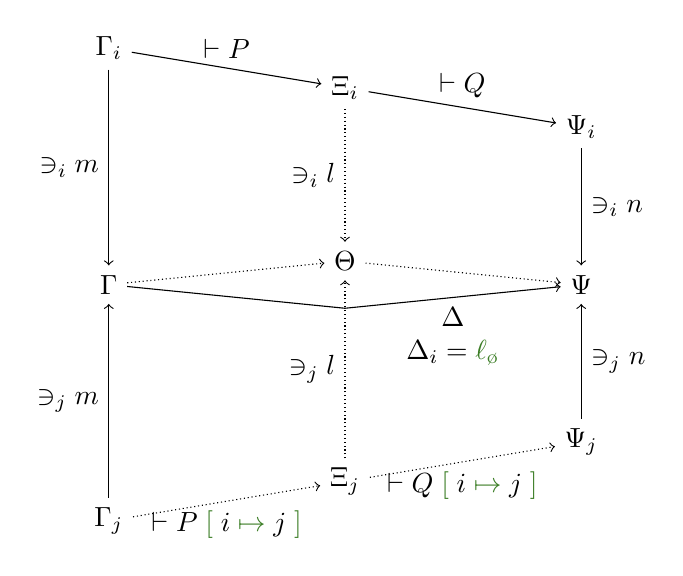
\begin{tikzpicture}
      \node (gamma-i) at (0,6)   {$\Gamma_i$};
      \node (gamma-m)   at (0,3)   {$\Gamma$};
      \node (gamma-j) at (0,0)   {$\Gamma_j$};
      \node (xi-i)    at (3,5.5) {$\Xi_i$};
      \node (theta)   at (3,3.3) {$\Theta$};
      \node (delta-m) at (3,2.7) {};
      \node (xi-j)    at (3,0.5) {$\Xi_j$};
      \node (psi-i)   at (6,5)   {$\Psi_i$};
      \node (psi-m)   at (6,3)   {$\Psi$};
      \node (psi-j)   at (6,1)   {$\Psi_j$};

      \draw[-]  (gamma-m) -- (delta-m.center);
      \draw[->] (delta-m.center) -- node[align=center,below] {$\Delta$\\$\Delta_i = \lz$}(psi-m);

      \draw[->,densely dotted] (gamma-m) -- (theta);
      \draw[->,densely dotted] (theta) -- (psi-m);
      
      \draw[->] (gamma-i) -- node[left] {$\ni_i m$} (gamma-m);
      \draw[->] (gamma-j) -- node[left] {$\ni_j m$} (gamma-m);
      \draw[->] (psi-i) -- node[right] {$\ni_i n$} (psi-m);
      \draw[->] (psi-j) -- node[right] {$\ni_j n$} (psi-m);

      \draw[->] (gamma-i) -- node[above] {$\vdash P$} (xi-i);
      \draw[->] (xi-i) -- node[above] {$\vdash Q$} (psi-i);
      \draw[->,densely dotted] (gamma-j) -- node[below] {$\vdash \subst{P}{j}{i}$} (xi-j);
      \draw[->,densely dotted] (xi-j) -- node[below] {$\vdash \subst{Q}{j}{i}$} (psi-j);
      \draw[->,densely dotted] (xi-i) -- node[left] {$\ni_i l$} (theta);
      \draw[->,densely dotted] (xi-j) -- node[left] {$\ni_j l$} (theta);
    \end{tikzpicture}
    \caption{
      Diagrammatic representation of the inductive substitution lemma.
      Continuous lines represent known facts, dotted lines proof obligations.
    }
    \label{fig:subst}
  \end{subfigure}
  \hspace{\fill} % DO NOT LEAVE EMPTY LINE
  \begin{subfigure}{.4\textwidth}
    \centering
    \begin{tikzpicture}
      \node (gamma-i) at (0,4)   {};
      \node (gamma-m) at (0,2)   {};
      \node (gamma-j) at (0,0)   {};
      \node (xi-i)    at (2,5)   {};
      \node (xi-m)    at (2,3.5) {};
      \node (xi-j)    at (2,2)   {};
      \node (psi-m)   at (4,3.5) {};

      \draw[->] (gamma-i) -- (xi-j);
      \draw[->] (gamma-m) -- (xi-j);
      \draw[->,densely dotted] (gamma-j) -- (xi-j);
      \draw[->] (gamma-i) -- (gamma-m);
      \draw[->] (gamma-j) -- (gamma-m);
      \draw[->] (xi-i)    -- (xi-m);
      \draw[->] (xi-j)    -- (xi-m);
      \draw[->] (xi-i)    -- (psi-m);
      \draw[->] (xi-m)    -- (psi-m);
      \draw[->,densely dotted] (xi-j)    -- (psi-m);
    \end{tikzpicture}
    \caption{
      Alternative approach without arrows $\ni_i n$ and $\ni_j n$.
      This approach makes composing typing derivations before and after substitution more difficult.
    }
    \label{fig:subst-alternative}
  \end{subfigure}
  \caption{Substitution with and without the \emph{adjustment} arrows $\ni_i n$ and $\ni_j n$}
\end{figure}

\begin{nitheorem}[Generalised substitution]
  \label{thm:subst-generalization}
  Let process $P$ be well-typed such that $\types{\gamma}{\Gamma_i}{P}{\Psi_i}$.
  The substituted variable $i$ has a usage $m$ in $\Gamma_i$, and a usage $n$ in $\Psi_i$.
  Substitution will take these usages $m$ and $n$ away from $i$ and transfer them to the variable $j$ we are substituting for.
  In other words, there must exist some $\Gamma$, $\Psi$, $\Gamma_j$ and $\Psi_j$ such that:
  \begin{multicols}{2}
  \begin{itemize}
    \item $\contains{\gamma}{\Gamma_i}{i}{t}{m}{\Gamma}$
    \item $\contains{\gamma}{\Gamma_j}{j}{t}{m}{\Gamma}$
    \item $\contains{\gamma}{\Psi_i}{i}{t}{n}{\Psi}$
    \item $\contains{\gamma}{\Psi_j}{j}{t}{n}{\Psi}$
  \end{itemize}
  \end{multicols}
  Let $\Gamma$ and $\Psi$ be related such that $\opctx{\Gamma}{\Delta}{\Psi}$ for some $\Delta$.
  Let $\Delta$ have a usage annotation $\lz$ at position $i$.
  Then substituting $i$ with $j$ in $P$ will be well-typed such that $\types{\gamma}{\Gamma_j}{\subst{P}{j}{i}}{\Psi_j}$.
  Refer to \autoref{fig:subst} for a diagramatic representation.
\end{nitheorem}

\begin{proof}
  By induction on $\types{\gamma}{\Gamma_i}{P}{\Psi_i}$.
  \begin{itemize}
    \item
      For constructor $\constr{end}$ observe that $\Gamma_i \equiv \Psi_i$ and thus $\Gamma_j \equiv \Psi_j$.
      The details are found in \autoref{app:subst-generalization}.

    \item
      For constructor $\constr{chan}$ we proceed inductively.
      
    \item
      For constructors $\constr{recv}$, $\constr{send}$ and $\constr{comp}$ we must find $\Theta$ in \autoref{fig:subst} and split the diagram along its vertical axis to proceed by induction.
      The details are found in \autoref{app:subst-generalization}.
  \end{itemize}  
\end{proof}

\begin{nitheorem}[Substitution]
  \label{thm:substitution}
  Let $P$ be a process typed under $\types{\gamma \comma t}{\Gamma \comma m}{P}{\Psi \comma \lz}$.
  Let $\ni_j m$ be a \textsc{VarRef} $\contains{\gamma}{\Psi}{j}{t}{m}{\Xi}$.
  Then, we can substitute the variable references to $\constr{0}$ in $P$ with $\suc j$ so that the result is well-typed under $\types{\gamma \comma t}{\Gamma \comma m}{\subst{P}{\suc j}{\constr{0}}}{\Xi \comma m}$.
\end{nitheorem}
\begin{proof}
  Use framing to derive $\contains{\gamma}{\Gamma}{j}{m}{\Theta}$ and $\types{\gamma \comma t}{\Theta \comma m}{P}{\Xi \comma \lz}$ for some $\Theta$.
  Supply these to the generalised \autoref{thm:subst-generalization}.
\end{proof}

\subsection{Subject Reduction}
\label{subject-reduction}
%%%%%%%%%%%%%%%%%%%%%%%%%%%%%%%%%%%%%%%%%%%%%%%%%%%%%%%%%%%%%%%%%%% 

\begin{nidefinition}
  For convenience, we use $\containsusage{\Gamma}{i}{x}{\Delta}$ to stand for $\contains{\gamma}{\Gamma}{i}{t}{x}{\Delta}$ for some $\gamma$ and $t$.
\end{nidefinition}

\begin{nitheorem}[Subject reduction]
  If $P$ reduces to $Q$ and $P$ is well-typed, then so is $Q$.
  In the \picalc{} we distinguish between a reduction $P \reduce{\constr{internal}} Q$ by communication on a channel created within $P$, and a reduction $P \reduce{\constr{external} \; i} Q$ by communication on a channel created outside of $P$.
  \begin{itemize}
    \item If the reduction is internal, we prove that if $\types{\gamma}{\Gamma}{P}{\Xi}$ then $\types{\gamma}{\Gamma}{Q}{\Xi}$.
    \item If the reduction is external and on channel $i$, we prove that if $\types{\gamma}{\Gamma'}{P}{\Xi}$ and $\containsusage{\Gamma'}{i}{\lio}{\Gamma}$ , then $\types{\gamma}{\Gamma}{Q}{\Xi}$.
  \end{itemize}
\end{nitheorem}

\begin{proof}
  By induction on the typing derivation on $P$.
  \hfill{}\\
  \begin{itemize}
    \item
    In the $\constr{comm}$ case we apply framing (\autoref{thm:framing}) to rearrange the assumptions and then apply substitution (\autoref{thm:substitution}) and strengthening (\autoref{thm:strengthening}).
  
    \item
    Reduction under $\constr{par}$ proceeds by induction on the process that is being reduced.

    \item
    Reduction under scope restriction case splits on the channel $c$ on which communication occurs.
    If $c$ is $\constr{internal}$ subject reduction proceeds inductively.
    If $c$ is $\constr{external}\; \constr{0}$ -- i.e. the channel that is being introduced by the scope restriction -- we use \autoref{lm:comm-capable} to subtract $\lio$ from the channel's usage annotation and then apply the induction hypothesis.
    If $c$ is $\constr{external}\; (\suc i)$ subject reduction proceeds inductively.

    \item
    In the $\constr{struct}$ case, we apply subject congruence (\autoref{thm:subject-congruence}) and the induction hypothesis.
  \end{itemize}
\end{proof}

%%%%%%%%%%%%%%%%%%%%%%%%%%%%%%%%%%%%%%%%%%%%%%%%%%%%%%%%%%%%%%%%%%% 
\section{Conclusion, Related and Future Work}

Leftover typing as presented in this paper is based on work by Allais \cite{Allais2018a}.
Allais uses leftover typing to mechanise in Agda a bidirectional type system for the linear \lambdacalc{}.
This type system sits on top of an untyped but well-scoped syntax with de Bruijn indices.
He proves type preservation and provides a decision procedure for type checking and type inference.
In this paper, we apply his technique to the \picalc{}, but limit ourselves to type-checking (scope restriction needs usage annotations) terms, and focus on generalising the usage algebra.
Drawing from quantitative type theory by McBride and Atkey \cite{McBride2016, Atkey2018}, it is crucial for us too to be able to talk about fully consumed resources.
As a by-product, we are able to transmit over a channel all none multiplicities of a fully exhausted channel over.

Recent years have seen an increase in the efforts to mechanise resource-aware concurrency calculi, but perhaps one of the earliest works is the formalisation of the linear \picalc{} in Isabelle/HOL by Gay \cite{Gay2001}.
Gay encodes the \picalc{} with linear and shared types into a more general framework.
As we do, he uses de Bruijn indices, a reduction relation and a type system posterior to the syntax.
However, in his work context splits are explicit, and the types of used multiplicities erased.

The work by Goto et al. \cite{Goto2016a} is likely the first formal contribution to session-types that comes along with a mechanised proof of type safety (in Coq). 
Their paper extends session types with polymorphism and pattern matching on session types.
They use a locally-nameless encoding of variable references, a syntax prior to types, and a LTS semantics that encodes session-typed processes into the \picalc{}.
Their type system uses reorering of contexts and extrinsic contex splits. 

Taking an intrinsic approach, Thiemann formalises in Agda the MicroSession (minimal GV \cite{}) calculus with support for recursion and subtyping \cite{Thiemann2019}.
Context splits are given extrinsically, and exhausted elements are removed from typing contexts altogether.
The semantics are given as an intrinsically typed CEK machine with a global context of session-typed channels.

Most recently, Rouvoet et al. provide an intrinsic encoding (where type safety follows by construction) of a \lambdacalc{} with session types \cite{Rouvoet2020}.
They use proof relevant separation logic and a notion of a supply and demand \emph{market} to make context splits transparent to the user.
Their separation logic is based on a partial commutative monoid that need not be functional nor cancellative.
Their typing rules preserve the balance between supply and demand, and are very elegant.
They distill their typing rules even further by modelling the supply and demand market as a state monad.


%%%%%%%%%%%%%%%%%%%%%%%%%%%%%%%%%%%%%%%%%%%%%%%%%%%%%%%%%%%%%%%%%%%
In this paper we provide a well-scoped syntax and a semantics for the \picalc{}, define on top of the syntax a type system capable of handling linear, gradual and shared types, and show that reduction preserves the well-typedness of a process.
We avoid the need for extrinsic context splits by defining a type system with leftovers \cite{Allais2018a}.
All this is mechanised in less than 1500 lines of code.

We consider proving that progress preserves the balancing of channels long-hanging fruit for the future.
More involved, we intend to add support for products and sum types to both the syntax and the type system.
Orthogonally, making our typing rules bidirectional would allows us to provide a decision procedure for type checking processes for a given set of algebras.
Following Erika Kreuer's suggestion, it might also be worth identifying an equivalence between our usage algebra and particular state machines.

\newpage
\bibliography{paper}

%%
\newpage
\appendix
%% Appendix
\section{Structural Congruence}
\label{app:struct}

Structural congruence is a congruent equivalence relation.
As such, rewrites can happen anywhere inside a process, and are closed under reflexivity, symmetry and transitivity as shown by the first row of \autoref{fig:struct-cong1}.
The rest of the rules defines structural congruence under a context $\mathcal{C}[\cdot]$ \cite{Sangio01}, respectively restriction, composition, input and output.

\begin{figure}[h]
  \begin{mathpar}
    \datatype
    { }
    {\Rec : \Set}
    \; \textsc{Rec}
  
    \inferrule
    { }
    {\constr{zero} : \Rec}
    
    \inferrule
    {r : \Rec}
    {\constr{one} \; r : \Rec}
  
    \inferrule
    {r \; s : \Rec}
    {\constr{two} \; r \; s : \Rec}
    
    \datatype
    {P \, Q : \Process_n \\ r : \Rec}
    {P \eq{r} Q : \Set}
    \; \textsc{Equals}
  
    \inferrule
    {eq : P \eqeq Q}
    {\constr{struct} \; eq : P \eq{\constr{zero}} Q}
  
    \inferrule
    {eq : P \eq{r} P'}
    {\constr{cong-scope} \; eq : \new P \eq{\constr{one} \; r} \new P'}
  
    \inferrule
    {eq : P \eq{r} P'}
    {\constr{cong-comp} \; eq : \comp{P}{Q} \eq{\constr{one} \; r} \comp{P'}{Q}}
  
    \inferrule
    {eq : P \eq{r} P'}
    {\constr{cong-recv} \; eq : \recv{x}P \eq{\constr{one} \; r} \recv{x}P'}
  
    \inferrule
    {eq : P \eq{r} P'}
    {\constr{cong-send} \; eq : \send{x}{y}P \eq{\constr{one} \; r} \send{x}{y}P'}
  
    \inferrule
    { }
    {\constr{refl} : P \eq{\constr{zero}} P}
  
    \inferrule
    {eq : P \eq{r} Q}
    {\constr{sym} \; eq : Q \eq{\constr{one} \; r} P}
  
    \inferrule
    {eq_1 : P \eq{r} Q \\ \; eq_2 : Q \eq{s} R}
    {\constr{trans} \; eq_1 \; eq_2 : P \eq{\constr{two} \; r \; s} R}
  \end{mathpar}
  \caption{Structural rewriting rules lifted to a congruent equivalence relation indexed by a recursion tree.}
  \label{fig:struct-cong1}
  \end{figure}

In the transitivity rule, we must show that if $P$ is structurally congruent to $Q$ and $Q$ is to $R$, and $P$ is well-typed, then so is $R$.
To do so, we need to proceed by induction and first get a proof of the well-typedness of $Q$, then use that to reach $R$.
To show the typechecker that the doubly recursive call terminates we index the equivalence relation $=$ by a type $\Rec$ that models the structure of the recursion.

\section{Usage Algebra}
\label{app:usage-algebra}

\todo{we haven't introduced the forall and implicit syntax}
\todo{introduce DEC and exists}

Our usage algebra is a ternary relation $\op{x}{y}{z}$ that is \emph{partial}, \emph{functional}, \emph{cancelative}, \emph{associtive}, and \emph{commutative}.
It has a \emph{neutral element} $\zero$ that is absorbed on either side, and that is also \emph{minimal}.
It has an element $\one$ that is used to count inputs and outputs.
These algebraic laws are defined as a record $\Quantifier_C$ on a carrier set $C$ in \autoref{fig:multiplicities}.
We use a terniary relation to model the partial monoidal operation.
We then encapsulate a set carriers and their algebras in \autoref{fig:indexed-multiplicities}.

\begin{figure}[h]
\begin{equation}
\begin{aligned}
  &\zero                  &:{} &                      &        & C \\
  &\one                   &:{} &                      &        & C \\
  &\op{\_}{\_}{\_}        &:{} &                      &        & C \to C \to C \to \Set \\
  &\func{\cdot-compute}  &:{} &\forall y z           & \to \; & \type{DEC} \; (\type{\exists} x . \; (\op{x}{y}{z})) \\
  &\func{\cdot-unique}   &:{} &\forall \{x x' y z\}  & \to \; & \op{x'}{y}{z} \to \op{x}{y}{z} \to x' \equiv x \\
  &\func{\cdot-unique^l} &:{} &\forall \{x y y' z\}  & \to \; & \op{x}{y'}{z} \to \op{x}{y}{z} \to y' \equiv y \\
  &\func{0\cdot-min^l}   &:{} &\forall \{y z\}       & \to \; & \op{\zero}{y}{z} \to y \equiv \zero \\
  &\func{\cdot-id^l}     &:{} &\forall \{x\}         & \to \; & \op{x}{\zero}{x} \\
  &\func{\cdot-comm}     &:{} &\forall \{x y z\}     & \to \; & \op{x}{y}{z} \to \op{x}{z}{y} \\
  &\func{\cdot-assoc}    &:{} &\forall \{x y z u v\} & \to \; & \op{x}{y}{z} \to \op{y}{u}{v} \to \type{\exists} w . \; (\op{x}{u}{w} \times \op{w}{v}{z})
\end{aligned}
\end{equation}
\caption{Quantifier algebra $\Quantifier_C$ algebra on a partial commutative monoid.}
\label{fig:multiplicities}
\end{figure}

\begin{figure}[h]
  \begin{equation}
    \begin{split}
      &\func{IDX}          &:{} &\Set \\
      &\func{\exists IDX}  &:{} &\func{IDX} \\
      &\func{USAGE}        &:{} &\func{IDX} \to \Set \\
      &\func{QUANTIFIERS}  &:{} &(i : \func{IDX}) \to \Quantifier_{\func{USAGE}_i}
    \end{split}
  \end{equation}
  \caption{Indexed set of usage algebras.}
  \label{fig:indexed-multiplicities}
\end{figure}

\section{Lemmas}
\label{app:lemmas}

\begin{nilemma}
  \label{lm:subst-unused}
  For every variables $i$ and $j$, if $i \not\equiv j$ then $\Unused_i (\subst{P}{j}{i})$.
\end{nilemma}
\begin{proof}
  By structural induction on \textsc{Process} and \textsc{Var}.
\end{proof}

\begin{nilemma}
  \label{lm:lower-lift}
  The function $\func{lower}_i \; P \; uP$ has an inverse $\func{lift}_i \; P$ that increments every $\textsc{Var}$ greater than or equal to $i$, such that $\func{lift}_i \; (\func{lower}_i \; P \; uP) \equiv P$.
\end{nilemma}
\begin{proof}
  By structural induction on \textsc{Process} and \textsc{Var}.
\end{proof}

\begin{nilemma}
  \label{lm:swap-swap}
  The function $\func{swap}_i \; P$ is its own inverse: $\func{swap}_i \; (\func{swap}_i \; P) \equiv P$.
\end{nilemma}
\begin{proof}
  By structural induction on \textsc{Process} and \textsc{Var}.
\end{proof}

\begin{nilemma}
  \label{lm:types-unused}
  For all well-typed processes $\types{\gamma}{\Gamma}{P}{\Xi}$, if the variable $i$ is unused within $P$, then $\Gamma$ at $i$ is equivalent to $\Xi$ at $i$.
\end{nilemma}
\begin{proof}
  By induction on \textsc{Process} and \textsc{Var}.
\end{proof}

\begin{nilemma}
  \label{lm:types-op}
  For all well-typed processes $\types{\gamma}{\Gamma}{P}{\Xi}$, there exists some $\Delta$ such that $\opctx{\Gamma}{\Delta}{\Xi}$.
\end{nilemma}
\begin{proof}
  By induction on \textsc{Process} and \textsc{Var}.
\end{proof}

\begin{nilemma}
  \label{lm:comm-capable}
  Every input usage context $\Gamma$ of a well-typed process $\types{\gamma}{\Gamma}{P}{\Delta}$ that reduces by communicating on a channel external to it (that is, $P \reduce{\constr{external} \; i} Q$ for some $Q$) has a multiplicity of at least $\lio$ at index $i$.
\end{nilemma}

\begin{proof}
  By induction on the reduction derivation $P \reduce{\constr{external \; i}}Q$.
\end{proof}
\end{document}
